\subsection{A numerical case study of the Edgeworth approximation}

To better understand the Edgeworth approximation, we investigate its behaviour when applied to a distribution for which the true density of the standardized sum is known. This is the case for the Gamma distribution as presented in \cite[Section 3.6]{kolassa2006series}.

\begin{example} \label{ex-gamma-edge}
    The Gamma distribution $\Gamma(p, \lambda)$ for $p, \lambda > 0$ has density
    \begin{equation*}
        f(x) = \frac{\lambda^p}{\Gamma(p)} x^{p-1} \expf{-\lambda x},
    \end{equation*}
    where $\Gamma$ is the Gamma function. Its characteristic function is $\zeta(t) = (1 - it/\lambda)^{-p}$. Hence, we can easily see that for $X_1, \ldots, X_n \simiid \Gamma(p, \lambda)$, both the sum and standardized mean of $X_1, \ldots, X_n$ follow a Gamma distribution with $\sum_{i=1}^n X_i \sim \Gamma(np, \lambda)$ and $n^{-1/2} \sum_{i=1}^n X_i \sim \Gamma(np, \lambda n^{-1/2})$. The cumulant generating function of the $\Gamma(p, \lambda)$ distribution is
    \begin{equation*}
        K(t) = p \logf{\lambda} - p\logf{\lambda - t},
    \end{equation*}
    hence the $(j)$-cumulant of $X$ is $\kappa_{(j)} = p\Gamma(j)\lambda^{-j}$. To be able to apply Theorem \ref{thm-edgeworth}, the density of the standardized sum must exist, which is true since we know that it follows a Gamma distribution.
    

    \begin{figure}[!htbp]
        \textbf{Density approximation of $\Gamma(p,1)$ standardized sums}
        \centering
        \subfloat[$p=1; n=1$\label{fig-single-gamma11}]{
            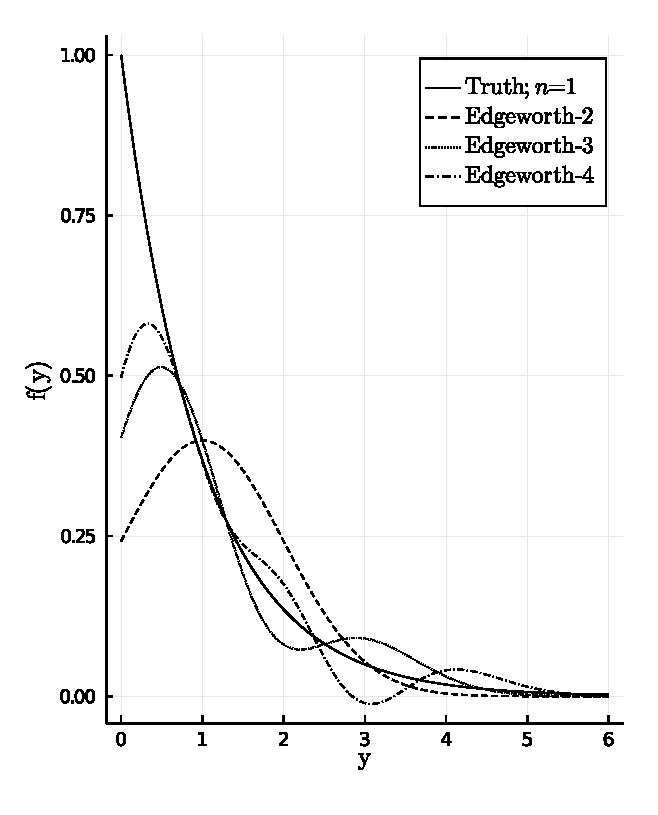
\includegraphics[width=8cm]{edgeworth_gamma11_1_terms.eps} 
        }
        \subfloat[$p=2; n=1$ \label{fig-single-gamma21}]{
            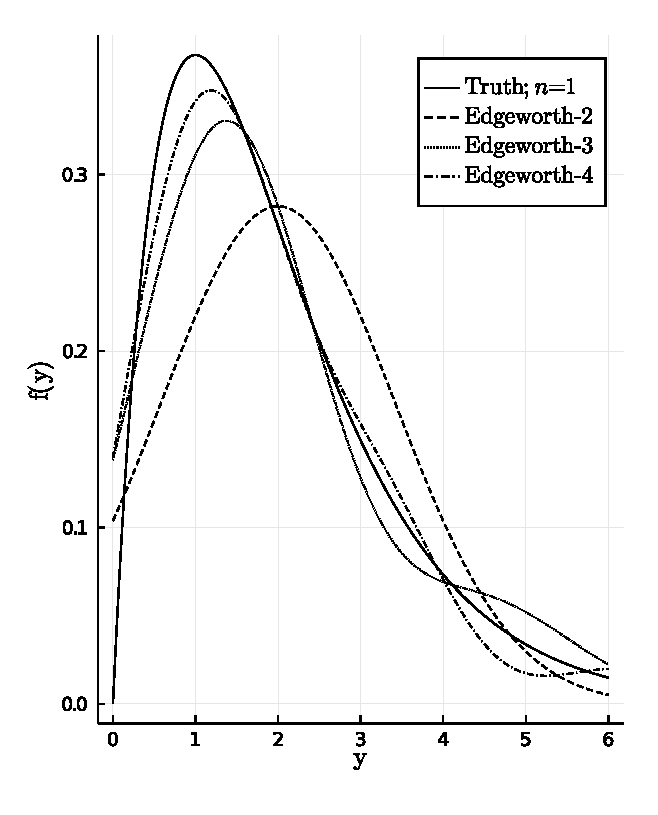
\includegraphics[width=8cm]{edgeworth_gamma21_1_terms.eps}
        }
        \qquad
        \subfloat[$p=1; n=10$ \label{fig-10-gamma11}]{
            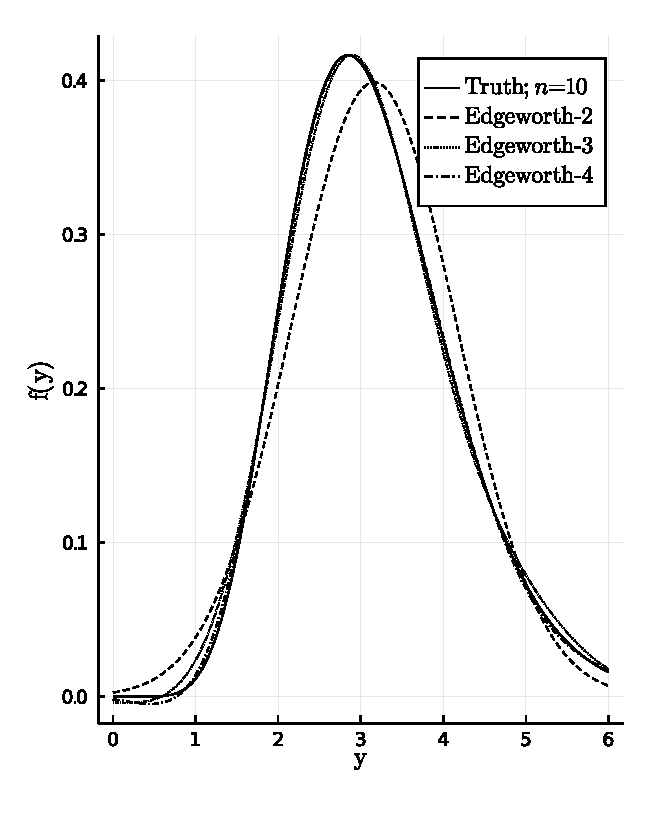
\includegraphics[width=8cm]{edgeworth_gamma11_10_terms.eps} 
        }
        \subfloat[$p=2; n=10$ \label{fig-10-gamma21}]{
            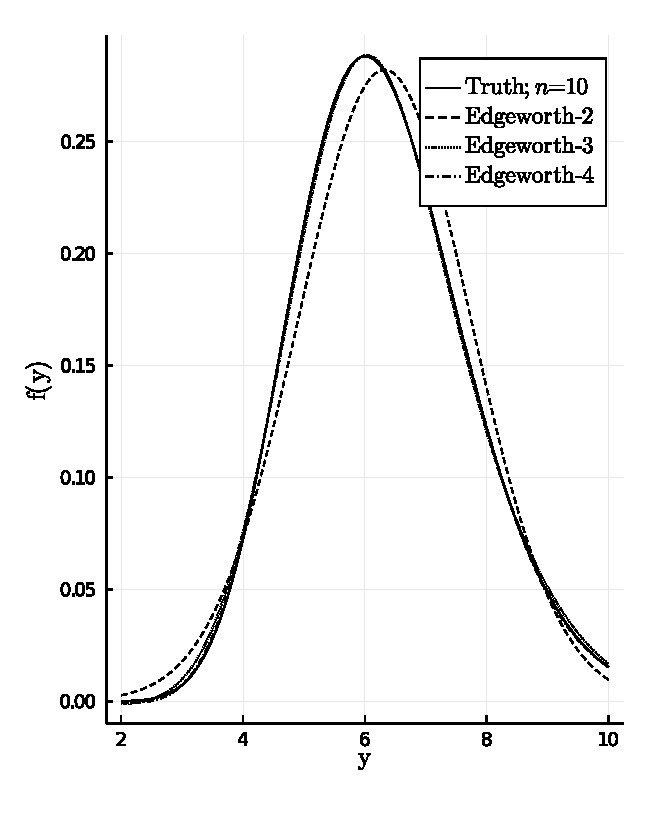
\includegraphics[width=8cm]{edgeworth_gamma21_10_terms.eps}
        }
        \caption{Several combinations of $p$ and $n$ exposing different behaviours of the Edgeworth approximation to the density of a standardized sum  of $n$ i.i.d.\,random variables following a $\Gamma(p, 1)$ distribution.}
        \label{fig-edgeworth}
    \end{figure}

    
    \begin{figure}[!htbp]
        \textbf{Approximation error of $\Gamma(p,1)$ standardized sums}
        \centering
        \subfloat[$p=1; n=1$\label{fig-err-abs-gamma11}]{
            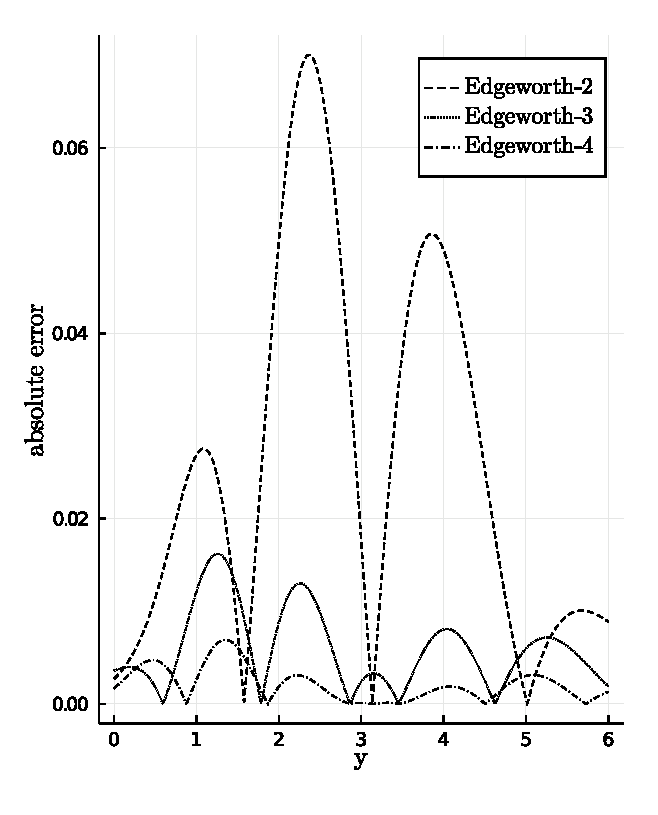
\includegraphics[width=7.5cm]{edgeworth_err_abs_gamma11_10_terms.eps} 
        }
        \subfloat[$p=2; n=1$ \label{fig-err-abs-gamma21}]{
            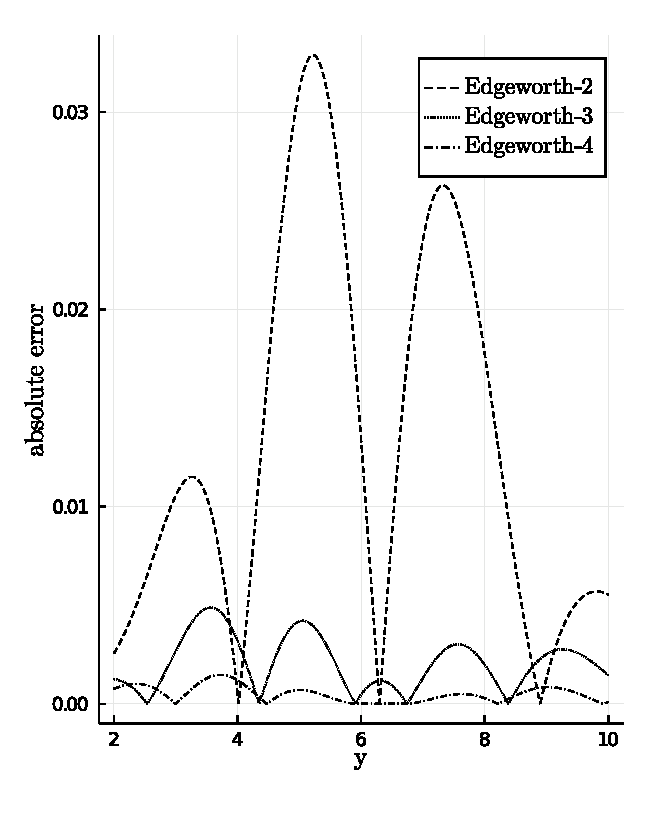
\includegraphics[width=7.5cm]{edgeworth_err_abs_gamma21_10_terms.eps} 
        }
        \qquad
        \subfloat[$p=1; n=10$ \label{fig-err-rel-gamma11}]{
            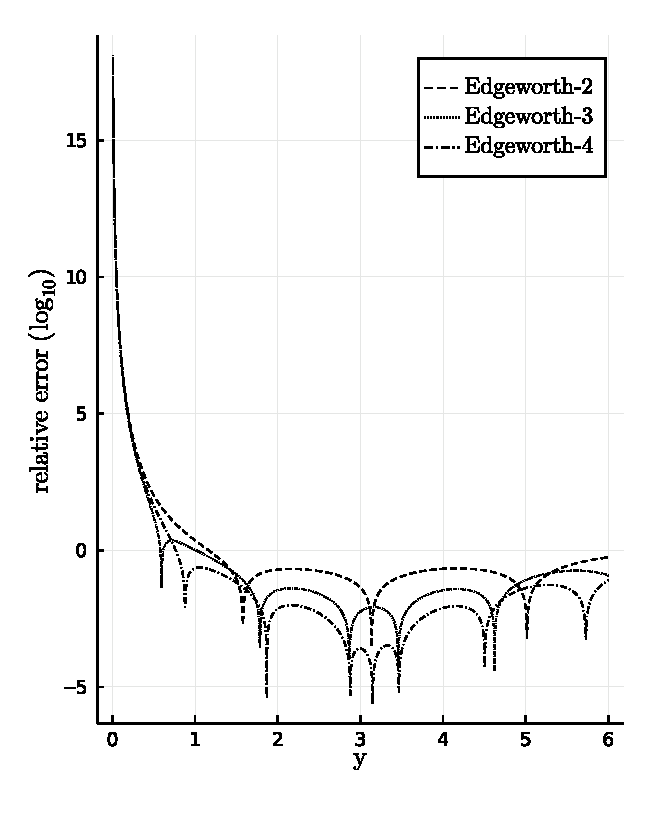
\includegraphics[width=7.5cm]{edgeworth_err_rel_gamma11_10_terms.eps}
        }
        \subfloat[$p=2; n=10$ \label{fig-err-rel-gamma21}]{
            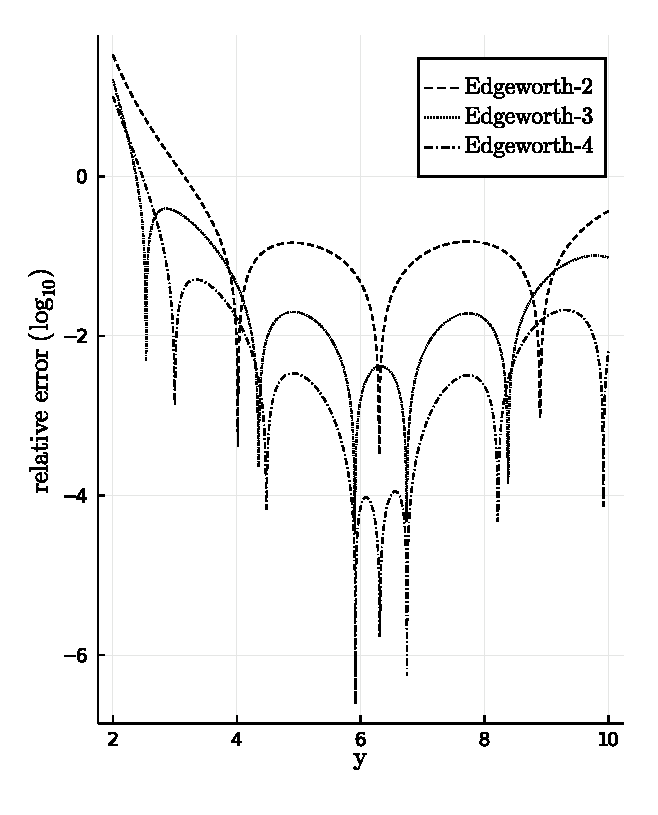
\includegraphics[width=7.5cm]{edgeworth_err_rel_gamma21_10_terms.eps}
        }
        \caption{Study of the approximation error of the Edgeworth approximation on a standardized sum of $n=10$ i.i.d.\,random variables following a $\Gamma(p, 1)$ distribution. The absolute error studied in Theorem \ref{thm-edgeworth} is well behaved as shown in the upper pane. However, the lower pane shows that the relative error of the approximation can be extremely high in low density regions where a low absolute error might still be a large relative error.}
        \label{fig-edgeworth-err}
    \end{figure}
    


    In Figure \ref{fig-edgeworth}, we show several examples of the behaviour of the Edgeworth approximation under different conditions. In the upper pane of Figure \ref{fig-edgeworth}, we compare the Edgeworth approximations of orders $k=2, 3, 4$ to the true density of a standardized sum of $n=1$ and $n=10$ random variables with a $\Gamma(p, 1)$ distribution for $p=1,2$. For $p=1$, $\Gamma(p, 1)$ is an exponential distribution. For $n = 1$, the discontinuity at $y = 0$ of the exponential distribution results in high oscillations of the Edgeworth approximation as demonstrated in Figure \ref{fig-single-gamma11} which even leads to negative values of the density approximation. Increasing to $p = 2$, we can see in Figure \ref{fig-single-gamma21} that the approximation is better behaved but unsurprisingly still does not well approximate the $\Gamma(2, 1)$ distribution. For both $p=1$ and $p=2$, increasing the number of terms summed to $n = 10$ results in seemingly good approximations to the density of the standardized sum as shown in Figures \ref{fig-10-gamma11} and \ref{fig-10-gamma21}.

    While Figure \ref{fig-edgeworth} appears to show good results of the Edgeworth approximation, it is hard to assess the quality of the approximations in regions of low probability. We display in Figure \ref{fig-edgeworth-err} the error of the Edgeworth series of orders $k=2,3,4$ approximating the density of a standardized sum of $n=10$ i.i.d.\,random variables following a $\Gamma(p, 1)$ distribution for $p=1$ and $p=2$. The upper pane demonstrates the control of the absolute approximation error studied in Theorem \ref{thm-edgeworth}. However, the lower pane of Figure \ref{fig-edgeworth-err} shows that the relative error can still reach very high values even as the order of the approximation increases. This is explained by the fact that even if the relative error is controlled, it might still be big relative to the true density in low probability regions.

    In many settings, one is interested in using distribution approximations to compute p-values in statistical tests. In this case, one is trying to find statistical evidence against a null hypotheses by demonstrating a low p-value of the null hypothesis model. Hence, the Edgeworth series itself can be ill suited for direct applications. However, as we will see in the next section, the Edgeworth approximation and related approximation results can still be used to construct approximations that are usable to estimate the density function in low probability regions.
\end{example}